%%%%%%%%%%%%%%%%%%%%%%%%%%%%%%%%%%%%%%%%%%%%%%%%%%%%%
%		CAP 5
%%%%%%%%%%%%%%%%%%%%%%%%%%%%%%%%%%%%%%%%%%%%%%%%%%%%%

\section[BMG poroso]{BMG poroso sinterizado}
\subsection{BMG poroso sinterizado}
%%%
% Introduccion
%%%

\begin{frame}
    \frametitle{Introducci\'on}
    \vspace{0.2cm}
%    \begin{itemize}
%        \item Metallic Glass: amorphous metal (without crystalline order).
%        \item Has advantages over crystalline metals, like elasticity combined with high resistance, strength and moldability.
%        \item Plasticity in these materials occurs by nucleation of shear transformation zones which grow into shear bands.
%        \item Shear bands may lead to brittle failure (heterogeneous deformation): importance of \textbf{preventing their propagation}.
%        \item A more homogeneous deformation may be achieved by adding \textbf{porosity}.
%    \end{itemize} 
    \begin{block}{Problem\'atica}
      Las bandas de corte pueden ocasionar la falla fr\'agil del material (deformaci\'on heterog\'enea).
    \end{block}
    \begin{block}{Posible soluci\'on}
     Una deformaci\'on m\'as homog\'enea puede lograrse al agregar porosidad.\\
     Similar al bloqueo del deslizamiento en metales cristalinos.
    \end{block}
\end{frame}

%%%
% Preparacion de la muestra
%%%

\begin{frame}
    \frametitle{Preparaci\'on de la muestra porosa}
    \vspace{0cm}
    \begin{enumerate}
        \item Ubicaci\'on aleatoria de part\'iculas de 2.5 nm de radio.
        \item Relajaci\'on @ 650K (volumen constante, pocos ps). 
        \item Hasta 10 ps de compresi\'on (400 bar).
        \item Se repiten los dos pasos anteriores.
        \item M\'as relajaci\'on: enfriado a temperatura 0, bar\'ostato a presi\'on 0, calentado hasta temperatura de simulaci\'on y bar\'ostato a presi\'on 0 (5 ps, temperatura constante)
        \begin{textblock*}{3cm}(2.5cm,6.5cm) % {block width} (coords)
            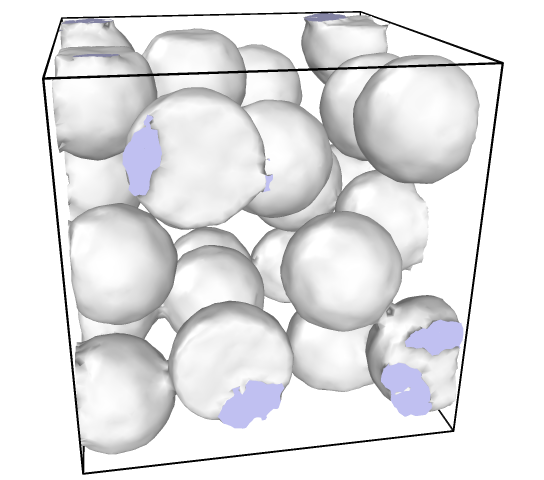
\includegraphics[width=3cm]{Cap_5/spheres2.png}
        \end{textblock*}
        \begin{textblock*}{3cm}(7cm,6.5cm) % {block width} (coords)
            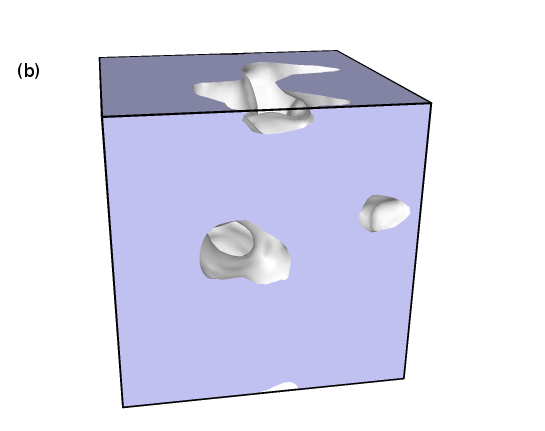
\includegraphics[width=3cm]{Cap_5/spheres3.png}
        \end{textblock*}
        \begin{textblock*}{3cm}(3.8cm,9.1cm)
         \scriptsize{Previo al sinterizado}
        \end{textblock*}
        \begin{textblock*}{3cm}(7.9cm,8.8cm)
         \scriptsize{Posterior al sinterizado}         
        \end{textblock*}
    \end{enumerate}
\end{frame}

%%%
% Resultados
%%%

\begin{frame}
    \frametitle{Detalles de la simulaci\'on}
    \vspace{0cm}
    \begin{itemize}
        \item Se crearon muestras con distintos niveles de porosidad (3.3\%, 5.8\% y 13.1\%).
        \item Velocidad de deformaci\'on 10$^9/s$, deformaci\'on puramente uniaxial.
        \item Condiciones de borde peri\'odicas.
    \end{itemize}
    \begin{textblock*}{12cm}(0.5cm,5cm)
      \begin{figure}[htp]
	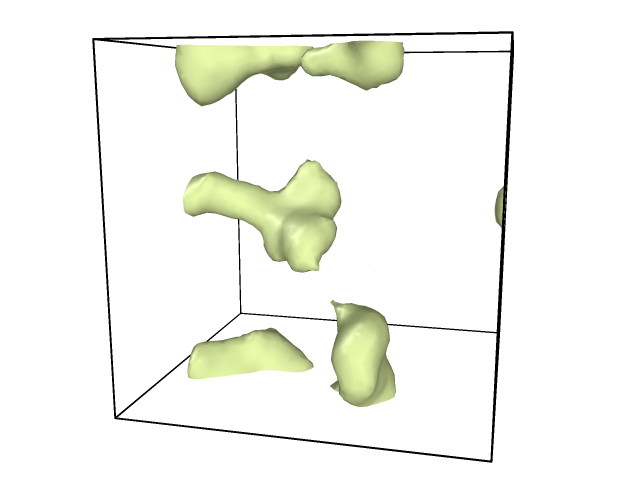
\includegraphics[width=4cm]{Cap_5/3_0strain.png}
	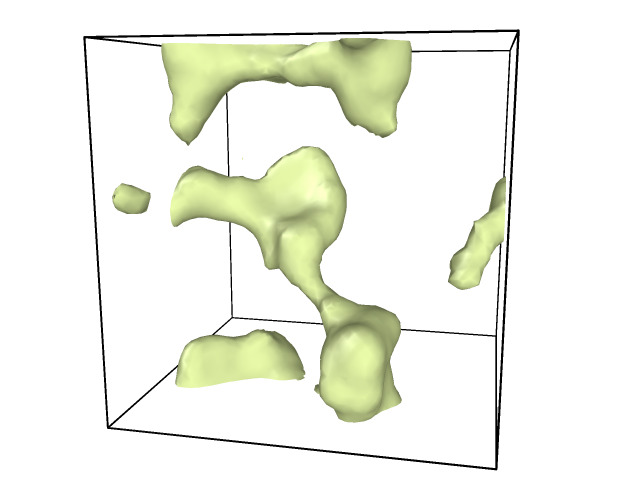
\includegraphics[width=4cm]{Cap_5/6_0strain.png}
	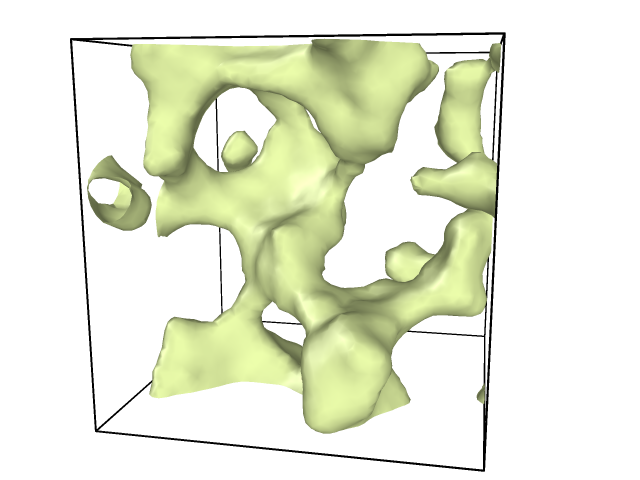
\includegraphics[width=4cm]{Cap_5/13_0strain_pores.png}
      \end{figure}
    \end{textblock*}
    \begin{textblock*}{2cm}(2.1cm,8.7cm)
      \scriptsize{3.3\%}
    \end{textblock*}
    \begin{textblock*}{2cm}(6.1cm,8.7cm)
      \scriptsize{5.8\%}
    \end{textblock*}
    \begin{textblock*}{2cm}(10.05cm,8.7cm)
      \scriptsize{13.1\%}
    \end{textblock*}
\end{frame}

\begin{frame}
 \frametitle{Resultados}
 \begin{textblock*}{12cm}(0.5cm,1.5cm)
  \begin{figure}[htp]
      \includegraphics[width=6cm]{Cap_5/SVF_strain_comp_dash.eps}
      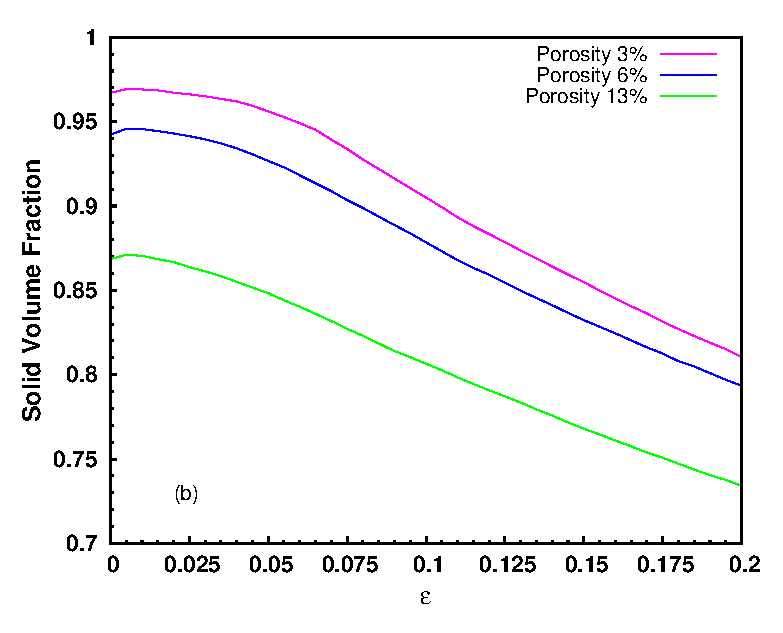
\includegraphics[width=6cm]{Cap_5/SVF_strain_tens.eps}
  \end{figure}
 \end{textblock*}
 \begin{textblock*}{6cm}(0.8cm,7cm)
  \centering
  \scriptsize{Compresi\'on}
 \end{textblock*}
 \begin{textblock*}{6cm}(6.8cm,7cm)
  \centering
  \scriptsize{Tracci\'on}
 \end{textblock*}
  \begin{textblock*}{\textwidth}(1cm,7.7cm)
  \centering
  Fracci\'on de volumen s\'olido vs deformaci\'on.\\
  El uso de condiciones peri\'odicas evita el cierre de poros en tracci\'on.
 \end{textblock*}
\end{frame}


\begin{frame}
    \frametitle{Resultados (compresi\'on)}
    \begin{textblock*}{7cm}(5.5cm,2cm) % {block width} (coords)
        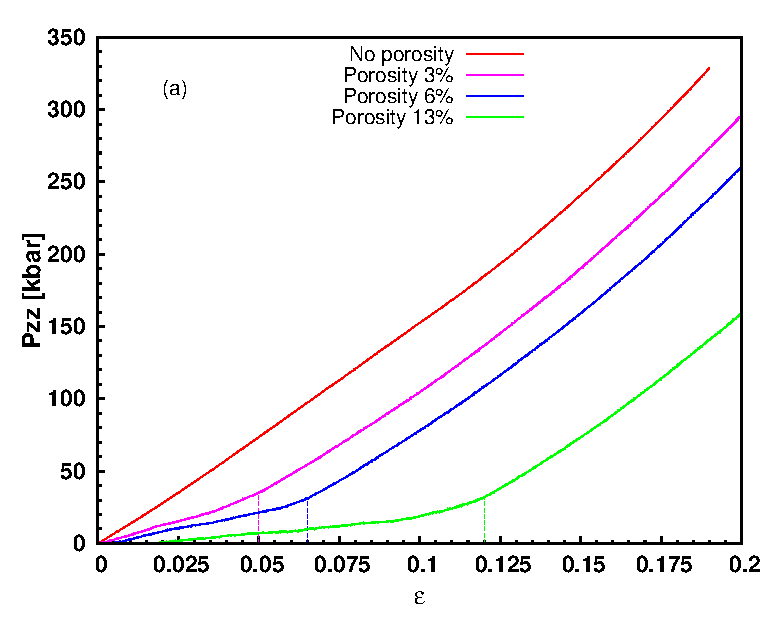
\includegraphics[width=7cm]{Presentacion_PANACM_Franco/Pzz_strain_comp_dash.eps}
    \end{textblock*}
    \begin{textblock*}{4.2cm}(5.8cm,6.4cm) % {block width} (coords)
        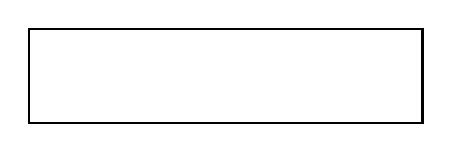
\begin{tikzpicture}
            \draw[thick] (0,0) rectangle (5cm,1.2cm);
        \end{tikzpicture}
    \end{textblock*}
    \begin{textblock*}{5cm}(0.6cm,2.2cm) % {block width} (coords)
        Los poros act\'uan como concentradores de tensi\'on, promoviendo la plasticidad. %Previo al colapso de los poros, la deformaci\'on aumenta, manteniendo bajos niveles de tensi\'on.
    \end{textblock*}
    \begin{textblock*}{4.5cm}(0.6cm,5cm) % {block width} (coords)
        Luego del colapso de los poros hay un endurecimiento significativo. %Indicar que todas las curvas son iguales
    \end{textblock*}
    \begin{textblock*}{12cm}(0.6cm,8.5cm) % {block width} (coords)
        A mayor porosidad $\rightarrow$ menor esfuerzo para cerrar los poros
    \end{textblock*}
\end{frame}

\begin{frame}
    \frametitle{Resultados (compresi\'on)}
    \begin{textblock*}{7cm}(5.5cm,2cm)
        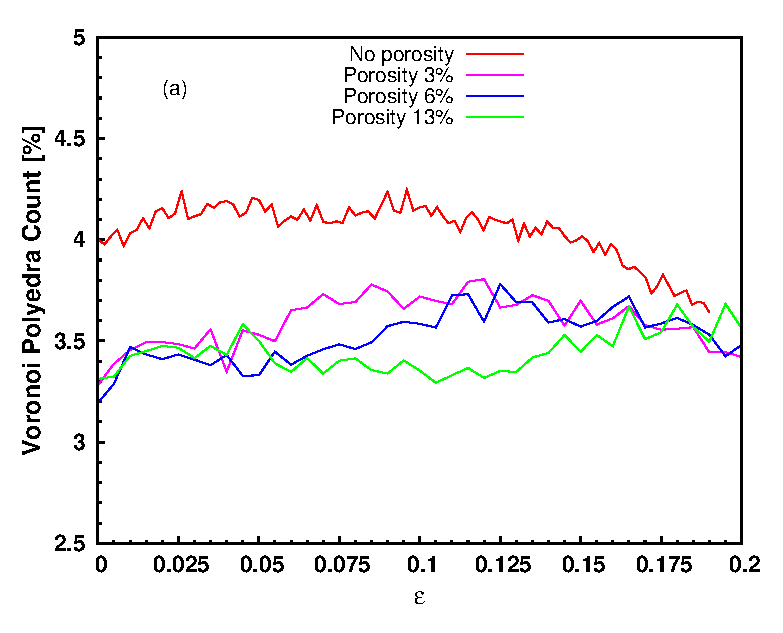
\includegraphics[width=7cm]{Presentacion_PANACM_Franco/tipe3_strain_comp.eps}
    \end{textblock*}
    \begin{textblock*}{4.8cm}(0.5cm,2.2cm)
        La ca\'ida en el n\'umero de \'atomos de Tipo 3 luego de una etapa constante ha sido considerada como un indicador del inicio de la plasticidad (Arman, 2010).
    \end{textblock*}
    \begin{textblock*}{4.8cm}(0.5cm,6.5cm)
        El resultado es contra-intuitivo.\\%Hay plasticidad pero los poliedros de Voronoi pr\'acticamente no cambian.\\
        Posible que hayan otros procesos involucrados.
    \end{textblock*}
\end{frame}

\begin{frame}
    \frametitle{Resultados (compresi\'on)}
    \begin{textblock*}{12cm}(0.4cm,1.7cm)
        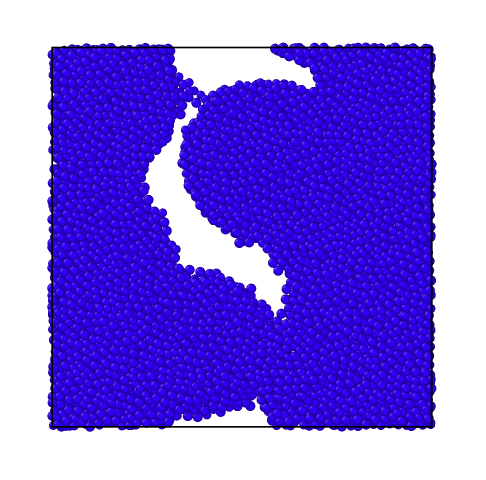
\includegraphics[width=4cm]{Cap_5/13_0strain.png}
        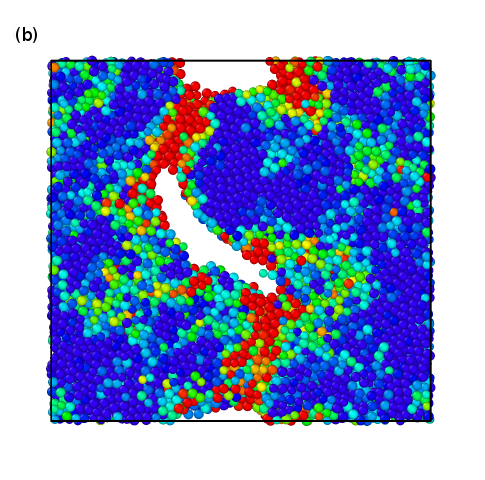
\includegraphics[width=4cm]{Cap_5/13_5strain_comp.png}
        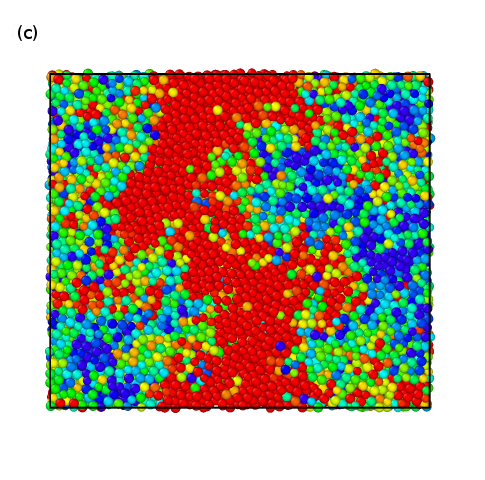
\includegraphics[width=4cm]{Cap_5/13_12strain_comp.png}\\
    \end{textblock*}
    \begin{textblock*}{12cm}(0.4cm,5.4cm)
     \centering
        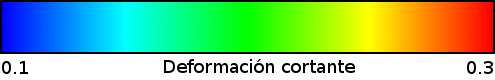
\includegraphics[width=4cm]{Cap_5/escala.png}
    \end{textblock*}
    \begin{textblock*}{12cm}(0.5cm,6.2cm)
        \centering
        \scriptsize{Porosidad 13\%. $\epsilon=$ 0, 5 y 12\%, respectivamente.}
    \end{textblock*}
    \begin{textblock*}{11cm}(1cm,7.1cm)
      \centering
        %Los poros act\'uan como concentradores de tensiones.\\
        Los poros impiden la propagaci\'on de bandas de corte.\\
        Bandas de corte nuclean diagonalmente en el espacio entre poros.
    \end{textblock*}
\end{frame}

\begin{frame}
    \frametitle{Resultados (tracci\'on)}
    \begin{textblock*}{7cm}(0.4cm,2cm) % {block width} (coords)
        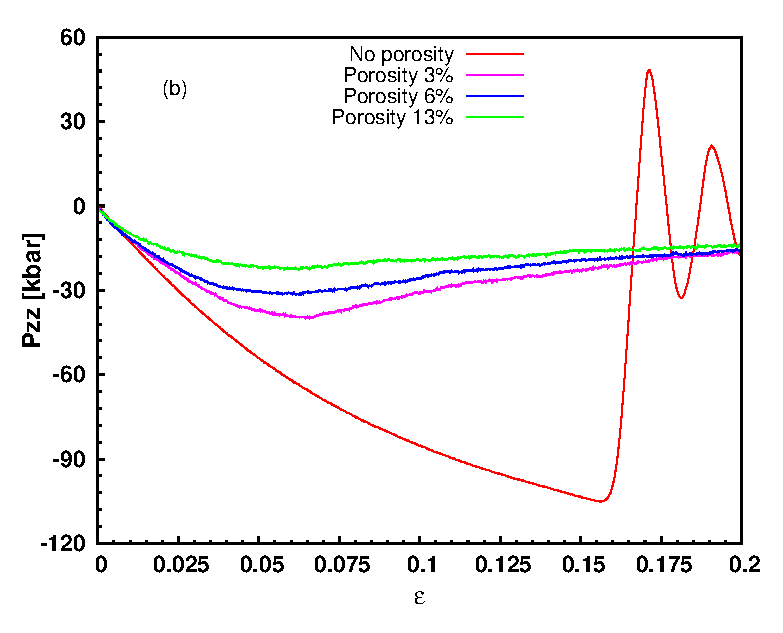
\includegraphics[width=7cm]{Cap_5/Pzz_strain_tens.eps}
    \end{textblock*}
    \begin{textblock*}{4cm}(8cm,2.2cm) % {block width} (coords)
        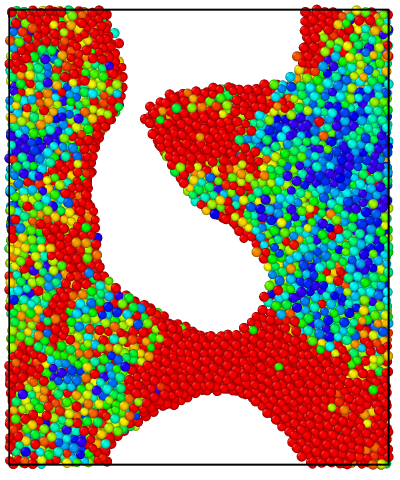
\includegraphics[width=4cm]{Presentacion_PANACM_Franco/13_20strain_tens_2.png}\\
        \centering
        \scriptsize{Deformaci\'on at\'omica.\\Porosidad 13\%, deformaci\'on 20\%.}
    \end{textblock*}
    \begin{textblock*}{11.5cm}(0.5cm,7.8cm) % {block width} (coords)
	\centering
        Flujo pl\'astico.\\
        El uso de condiciones de borde peri\'odicas evita el cierre de poros (no hay estricci\'on).
    \end{textblock*}
\end{frame}

\begin{frame}
    \frametitle{Resultados (tracci\'on)}
    \begin{textblock*}{12cm}(0.4cm,2cm) % {block width} (coords)
        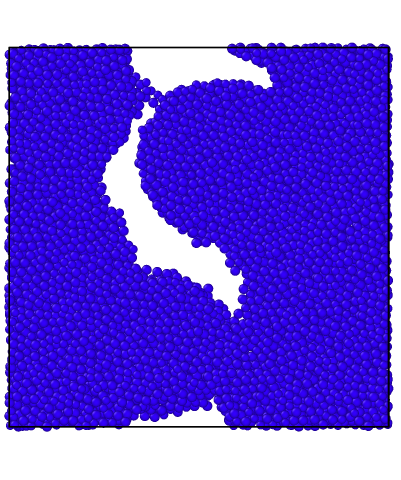
\includegraphics[width=4cm]{Presentacion_PANACM_Franco/13_0strain.png}
        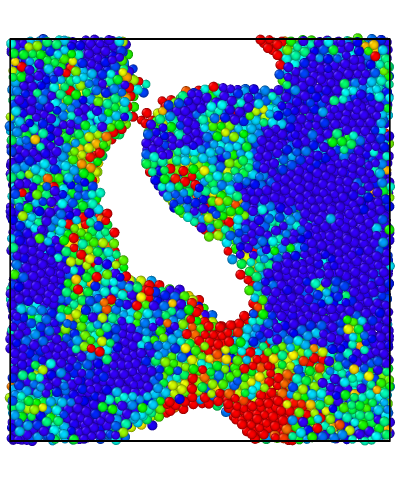
\includegraphics[width=4cm]{Presentacion_PANACM_Franco/13_6strain_tens.png}
        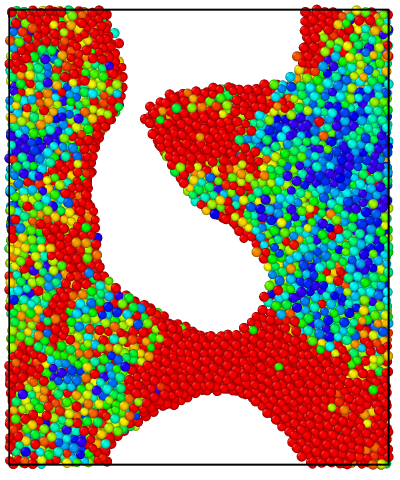
\includegraphics[width=4cm]{Presentacion_PANACM_Franco/13_20strain_tens_2.png}
    \end{textblock*}
    \begin{textblock*}{12cm}(0.4cm,6.9cm)
     \centering
        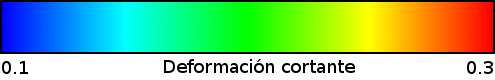
\includegraphics[width=4cm]{Cap_5/escala.png}
    \end{textblock*}
    \begin{textblock*}{12cm}(0.5cm,7.7cm)
        \centering
        \scriptsize{Porosidad 13\%. $\epsilon=$ 0, 6 y 20\%, respectivamente.}
    \end{textblock*}
    \begin{textblock*}{11.5cm}(1cm,8.5cm) % {block width} (coords)
    \centering
	La deformaci\'on cortante se concentra principalmente alrededor de los poros.
%            \item Relative position between atoms remains almost the same.
    \end{textblock*}
\end{frame}

\begin{frame}
    \frametitle{Resultados (tracci\'on)}
    \begin{textblock*}{7.5cm}(0.3cm,2cm) % {block width} (coords)
        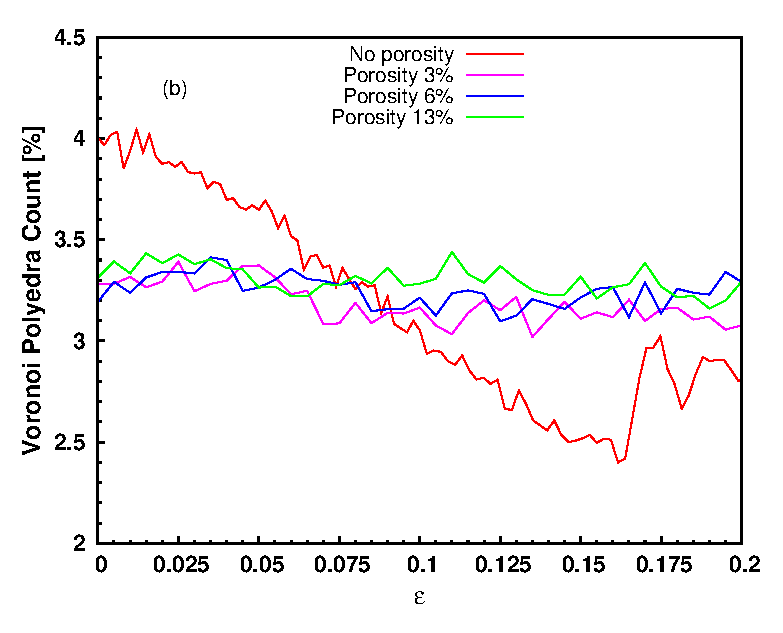
\includegraphics[width=7.5cm]{Presentacion_PANACM_Franco/tipe3_strain_tens.eps}
    \end{textblock*}
    \begin{textblock*}{4.2cm}(6.7cm,4cm) % {block width} (coords)
        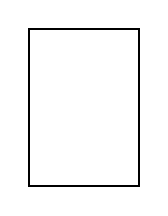
\begin{tikzpicture}
            \draw[thick] (0,0) rectangle (1.4cm,2cm);
        \end{tikzpicture}
    \end{textblock*}
    \begin{textblock*}{5cm}(8cm,3cm) % {block width} (coords)
        Constante luego de la nucleaci\'on del void.
    \end{textblock*}
    \begin{textblock*}{12cm}(0.4cm,7.9cm) % {block width} (coords)
    \centering
	Se facilita el movimiento de \'atomos alrededor de los poros.\\
	Esto evita la formaci\'on de STZ fuera de los alrededores de los poros.
    \end{textblock*}
\end{frame}

%%%
% Conclusiones
%%%

%\begin{frame}
    %\frametitle{Conclusions}
    %\vspace{0.5cm}
    %\begin{itemize}
        %\item Sintering process leads to glass with taylored porosity values.
        %\item Under compression: pores act as stress concentrators but also delay nucleation of SBs. After closure, there is hardening.
        %\item Under tension: pores do not close and they concentrate plastic flow around them, also impeding formation of STZ and SBs.
        %\item Results under strain were somewhat comparable to the ones by Yuan et al. (2014), where a single crystal sample with voids was studied.
    %\end{itemize}
    %\begin{textblock*}{12cm}(1cm,8.8cm) % {block width} (coords)
        %\scriptsize{Yuan F. and Wu X., \textit{AIP ADVANCES}, \textbf{4}, 127109 (2014).}
    %\end{textblock*}
%\end{frame}

%\begin{frame}
    %\begin{textblock*}{5cm}(2cm,3.2cm) % {block width} (coords)
        %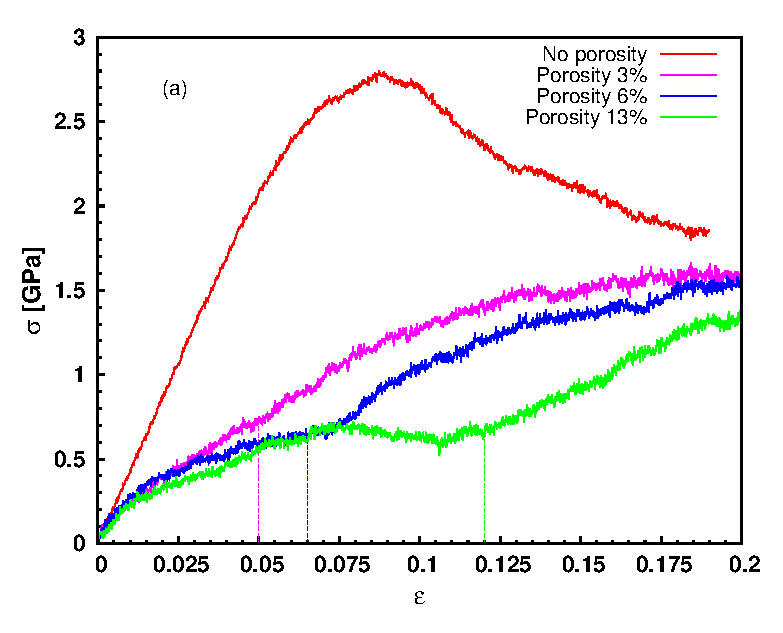
\includegraphics[width=5cm]{Presentacion_PANACM_Franco/stress_strain_comp_dash.eps}
    %\end{textblock*}
    %\begin{textblock*}{3cm}(7cm,3cm) % {block width} (coords)
        %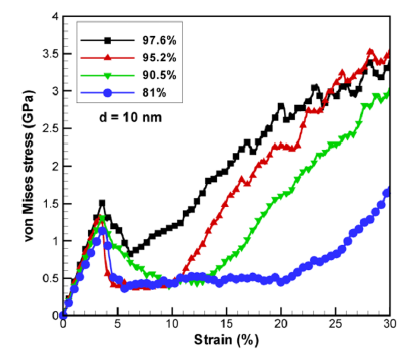
\includegraphics[width=5cm]{Presentacion_PANACM_Franco/Yuan_VM.png}
    %\end{textblock*}
    %\begin{textblock*}{12cm}(1cm,8.2cm) % {block width} (coords)
        %\small{Yuan F. and Wu X., \textit{AIP ADVANCES}, \textbf{4}, 127109 (2014).}
    %\end{textblock*}
%\end{frame}

%\begin{frame}
    %\begin{textblock*}{5cm}(2cm,3.2cm) % {block width} (coords)
        %\includegraphics[width=5cm]{Presentacion_PANACM_Franco/SVF_strain_comp_dash.eps}
    %\end{textblock*}
    %\begin{textblock*}{3cm}(7cm,3cm) % {block width} (coords)
        %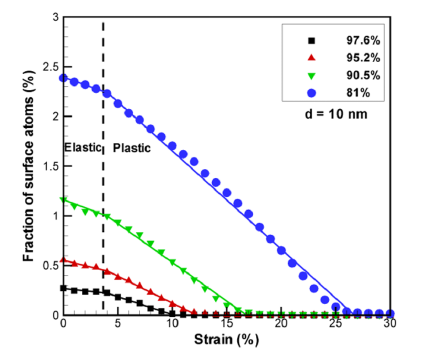
\includegraphics[width=5cm]{Presentacion_PANACM_Franco/Yuan_SVF.png}
    %\end{textblock*}
    %\begin{textblock*}{12cm}(1cm,8.2cm) % {block width} (coords)
        %\small{Yuan F. and Wu X., \textit{AIP ADVANCES}, \textbf{4}, 127109 (2014).}
    %\end{textblock*}
%\end{frame}

\begin{frame}
 \frametitle{Influencia velocidad de enfriamiento}
 Se modifica la velocidad de enfriamiento/calentamiento de $6.5 \cdot 10^{14} K/s$ a $6.5 \cdot 10^{12} K/s$

 \only<1>{
 \begin{textblock*}{6cm}(0.5cm,3cm)
  \centering
  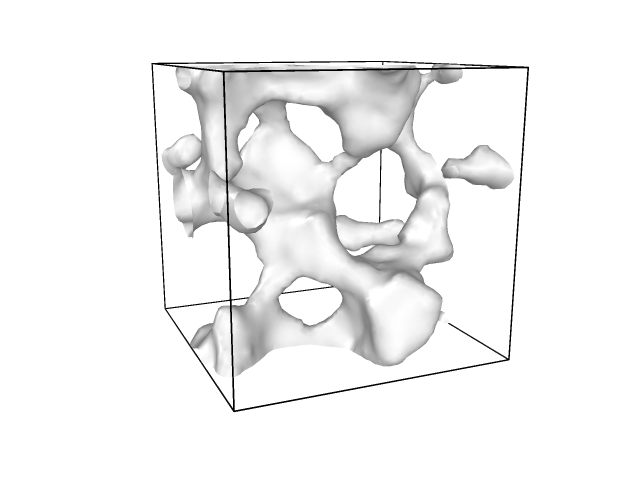
\includegraphics[width=6cm]{Cap_5/porosidad13_vel14_strain0.png}
 \end{textblock*}
 \begin{textblock*}{6cm}(0.5cm,7.1cm)
  \centering
  \scriptsize{$6.5 \cdot 10^{14} K/s$, porosidad 13.1\%}
 \end{textblock*}   

 \begin{textblock*}{6cm}(6.5cm,3cm)
  \centering
  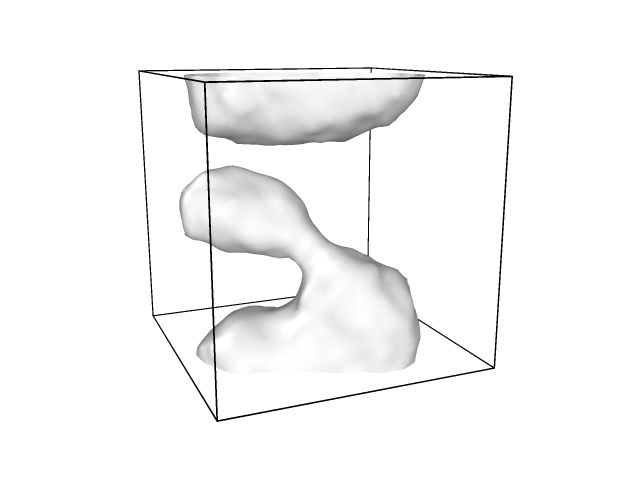
\includegraphics[width=6cm]{Cap_5/porosidad13_vel12_strain0.png}
 \end{textblock*}   
 \begin{textblock*}{6cm}(6.5cm,7.1cm)
  \centering
  \scriptsize{$6.5 \cdot 10^{12} K/s$, porosidad 13.5\%}
 \end{textblock*}   
 
 
 \begin{textblock*}{10cm}(1.2cm,8cm)
  \centering
  Cambia la forma de los poros (disposiciones de menor energía).
 \end{textblock*}

    %\caption[Comparación de muestras con velocidades de enfriamiento/calentamiento distintas (porosidad 13\%)]{Estado inicial de las muestras generadas con velocidades de enfriamiento/calentamiento diferentes, para el caso de porosidad 13\%.}
}
 
 \only<2>{
 \begin{textblock*}{12cm}(0cm,2.6cm)
    \begin{figure}[htp]
    \centering
    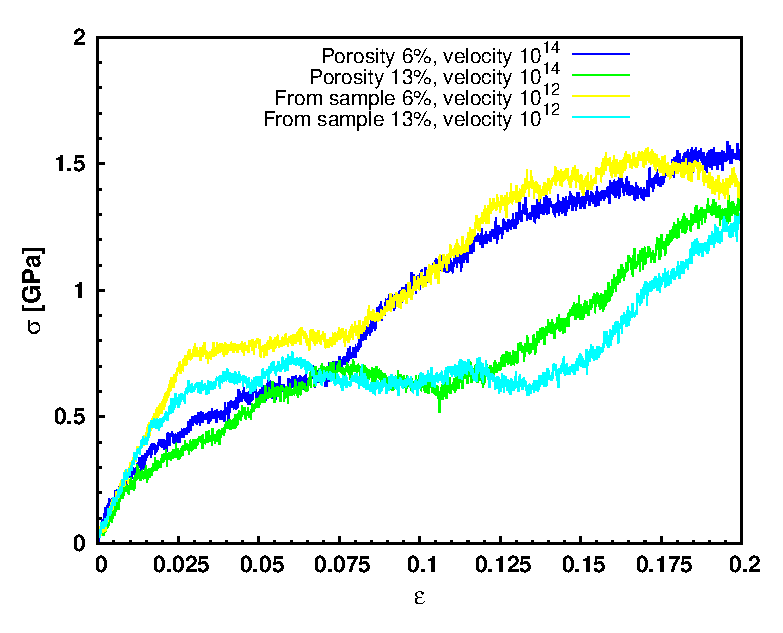
\includegraphics[width=6cm]{Cap_5/porosity_VM_strain_comp_vel12.eps}
    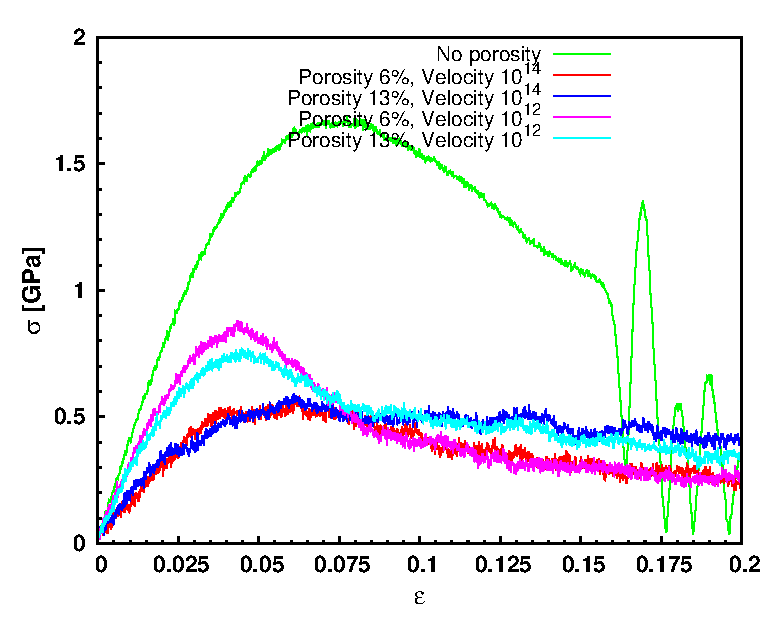
\includegraphics[width=6cm]{Cap_5/porosity_VM_strain_trac_vel12.eps}
    %\caption[Tensión de Von Mises vs deformación, velocidades $10^{12} K/s$ y $10^{14} K/s$]{Tensión de Von Mises vs deformación. Velocidad de enfriamiento/calentamiento de $6.5 \cdot 10^{12} K/s$}
    \end{figure}
 \end{textblock*}
 \begin{textblock*}{6cm}(1cm,7.1cm)
  \centering
  \scriptsize{Compresión}
 \end{textblock*}
 \begin{textblock*}{6cm}(5cm,7.1cm)
  \centering
  \scriptsize{Tracción}
 \end{textblock*}
 \begin{textblock*}{12cm}(1cm,8.2cm)
 Aumenta $\sigma$ máxima soportada y módulo de elasticidad.\\
 Luego de 7.5\% es dependiente del SVF. 
 \end{textblock*}
 
}

\end{frame}

\begin{frame}
 \frametitle{Influencia ubicaci\'on de poros}
 
  Se realiza un segundo sinterizado con una distribución de partículas diferente

 \only<1>{
 \begin{textblock*}{6cm}(0.5cm,3cm)
  \centering
  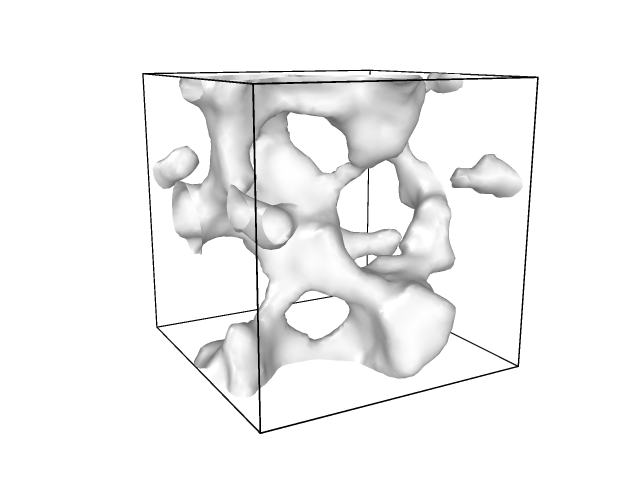
\includegraphics[width=6cm]{Cap_5/PrimerSintering_13_0strain.png}
 \end{textblock*}
 \begin{textblock*}{6cm}(0.5cm,7.25cm)
  \centering
  \scriptsize{Primer sinterizado, porosidad 13\%}
 \end{textblock*}   

 \begin{textblock*}{6cm}(6.5cm,3cm)
  \centering
  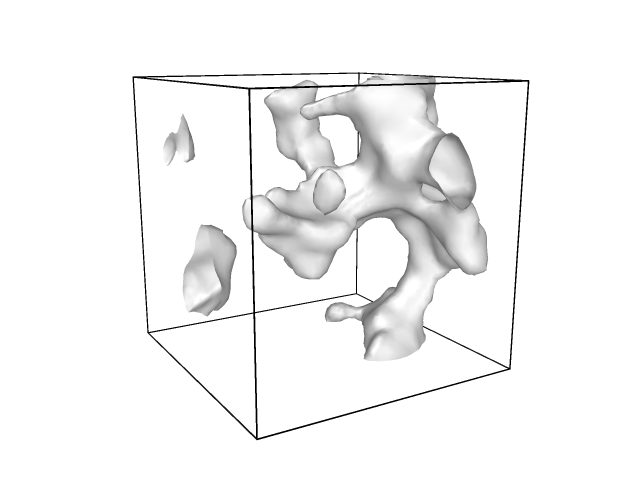
\includegraphics[width=6cm]{Cap_5/SegundoSintering_13_0strain.png}
 \end{textblock*}   
 \begin{textblock*}{6cm}(6.5cm,7.25cm)
  \centering
  \scriptsize{Segundo sinterizado, porosidad 13\%}
 \end{textblock*}   
 
 
 \begin{textblock*}{10cm}(1.2cm,8cm)
  \centering
  La distribución de poros es aleatoria.
 \end{textblock*}

    %\caption[Comparación de muestras con velocidades de enfriamiento/calentamiento distintas (porosidad 13\%)]{Estado inicial de las muestras generadas con velocidades de enfriamiento/calentamiento diferentes, para el caso de porosidad 13\%.}
}
 
 \only<2>{
 \begin{textblock*}{12cm}(0.3cm,2.6cm)
    \begin{figure}[htp]
    \centering
    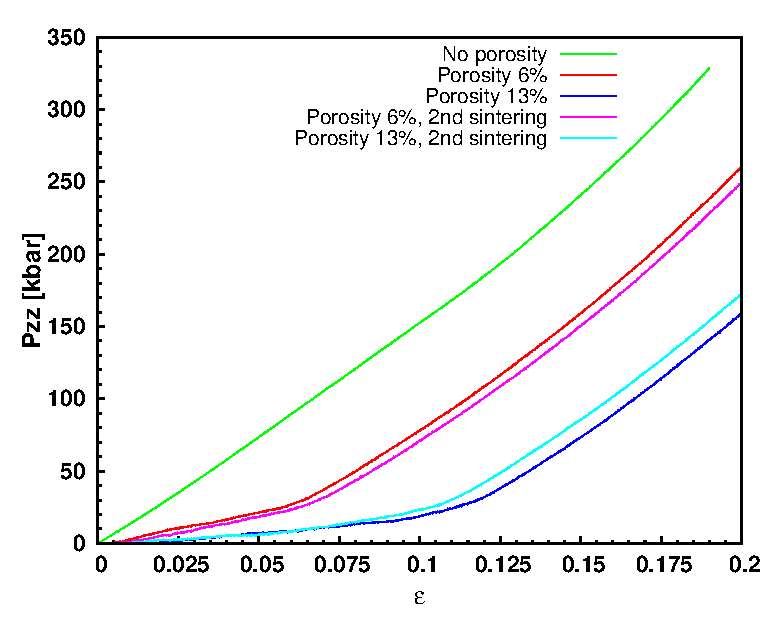
\includegraphics[width=6cm]{Cap_5/porosity_PZZ_strain_comp_2sintering.eps}
    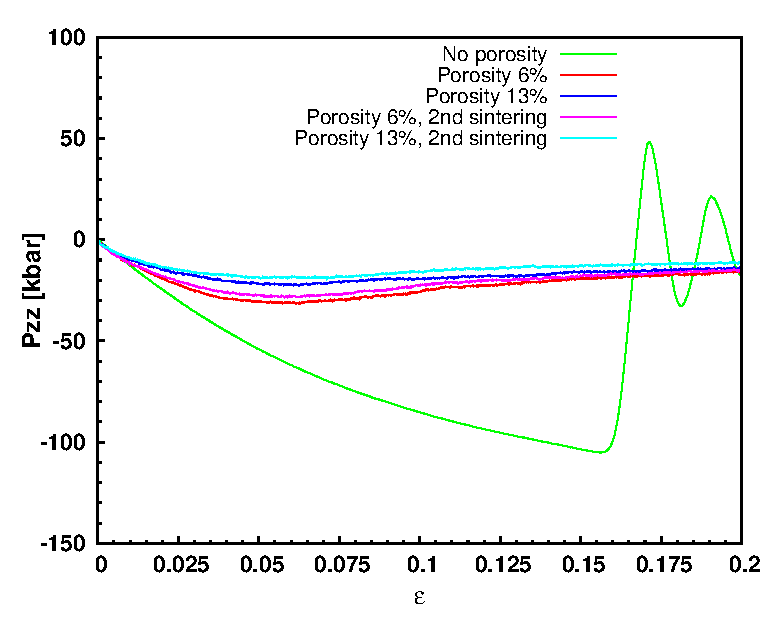
\includegraphics[width=6cm]{Cap_5/porosity_PZZ_strain_trac_2sintering.eps}
    %\caption[Tensión de Von Mises vs deformación, velocidades $10^{12} K/s$ y $10^{14} K/s$]{Tensión de Von Mises vs deformación. Velocidad de enfriamiento/calentamiento de $6.5 \cdot 10^{12} K/s$}
    \end{figure}
 \end{textblock*}
 \begin{textblock*}{6cm}(1.9cm,7.1cm)
  \centering
  \scriptsize{Compresión}
 \end{textblock*}
 \begin{textblock*}{6cm}(5.3cm,7.1cm)
  \centering
  \scriptsize{Tracción}
 \end{textblock*}
 \begin{textblock*}{12cm}(0.5cm,8.2cm)
 Comportamiento dependiente del SVF y no de la ubicación de los poros. 
 \end{textblock*}
 }
\end{frame}
